\documentclass[aspectratio=169]{beamer}
\usetheme{Frankfurt}
\usepackage{tikz}
\usepackage{minted}
\usepackage{pdfpages}
\usefonttheme{professionalfonts}
\usecolortheme{sidebartab}
\usepackage{xcolor}
\usepackage{svg}
\usepackage{hyperref}
\definecolor{bg}{RGB}{210, 255, 180}
\definecolor{aquamarine}{rgb}{0.5, 1.0, 0.83}
\newcommand{\highlight}[1]{\colorbox{pink}{#1}}
\newcommand{\highlightcode}[1]{\colorbox{bg}{#1}}
\newcommand{\highlightflag}[1]{\colorbox{yellow}{#1}}
\newcommand{\colorprog}[1]{\colorbox{aquamarine}{#1}}
\newcommand{\colorpred}[1]{\colorbox{green}{#1}}
\newcommand{\colorinv}[1]{\colorbox{yellow}{#1}}
\newcommand{\coloralg}[1]{\colorbox{lg}{#1}}
\newcommand{\coloryellow}[1]{\colorbox{yellow}{#1}}
\usetikzlibrary{chains, shadows.blur, trees}
%Information to be included in the title page:
\title[\url{https://google.com}] %optional
{The Hot Path SSA Form in LLVM}

\subtitle{Algorithms \& Applications}

\author[VIP1 \& VIP2] % (optional, for multiple authors)
{IIT Kanpur \\ Dept. Of Computer Science \& Engineering}

\institute[IDK] % (optional)
{
	\inst{1}%
	IIT Kanpur\\
	PRAISE Group
}

\date[01/03/2022] % (optional)
{Mohd. Muzzammil, Abhay Kumar, Sumit Lahiri \\ Dr. Awanish Pandey, Dr. Subhajit Roy}

\AtBeginSection[]
{
	\begin{frame}<beamer>
		\frametitle{Presentation Outline : Section \thesection}
		\tableofcontents[
			currentsection,
			hideothersubsections,
			currentsubsection
		]
	\end{frame}
}


\begin{document}
\frame{\titlepage}

\footnotesize
\section{HPSSA : Why another SSA Form?}
\subsection{Profile Guided Optimization}
{
	\setbeamercolor{background canvas}{bg=}
	\includepdf[pages={3,4,5,6,7,8,9,10,11,12,13,14,15,18}]{summary.pdf}
}
\subsection{Doing Profile Guided Optimizations is Hard!}
{
	\setbeamercolor{background canvas}{bg=}
	\includepdf[pages={18}]{summary.pdf}
}
\begin{frame}[fragile]
	\frametitle{Profile Guided Optimization is easy with HPSSA Form}
	\begin{columns}
		\begin{column}{0.4\textwidth}
	\begin{minted}[xleftmargin=1em, tabsize=2, numbersep=0.5em, escapeinside=||, fontsize=\tiny, linenos, highlightcolor=yellow, highlightlines={}]{cpp}
// Function to process "llvm.tau" function intrinsic.
visitTauNode() {
	...
	SpecValueLatticeElement TauState = getValueState(&Tau), 
		beta = getValueState(Tau.getOperand(1)), 
		x0 = getValueState(Tau.getOperand(0));
	if (TauState.isOverdefined())
		return (void)markOverdefined(&Tau);
	for (unsigned i = 1, e = (Tau.getNumOperands() - 1); i != e; ++i) {
		SpecValueLatticeElement IV = getValueState(Tau.getOperand(i));
		beta.mergeIn(IV);
		NumActiveIncoming++;
		if (beta.isOverdefined())
		break;
	}
	
	beta.mergeIn(x0);
	if (beta.isConstant())
		TauState.markSpeculativeConstant(beta.getConstant());
	
	if (beta.isConstantRange())
		TauState.markSpeculativeConstantRange(beta.getConstantRange());
	
	if (beta.isOverdefined() || x0.isOverdefined())
		TauState.markOverdefined();
	...
}
\end{minted}
		\end{column}
	\begin{column}{0.05\textwidth} \end{column}
		\begin{column}{0.3\textwidth}  
			\begin{minted}[fontsize=\tiny, xleftmargin=1em, tabsize=2, numbersep=0.5em, linenos, highlightcolor=yellow, highlightlines={10}]{cpp}
// Omit handling of "llvm.tau" intrinsic 
// as a regular Instruction.
for (auto& I : *&(*(BB))) {
	CallInst* CI = dyn_cast<CallInst>(&I);
	if (CI != NULL) {
		Function* CF = CI->getCalledFunction();
		if (CF != NULL &&
		CF->getIntrinsicID() == 
			Function::lookupIntrinsicID("llvm.tau")) {
			visitTauNode(I);
		} else {
			visit(I);
		} 
	} else {
		visit(I);
	}
}
			\end{minted}
		\end{column}
	\end{columns}
\end{frame}
\begin{frame}[fragile]
	\frametitle{Using \texttt{HPSSAPass} [It is easy!]}
	\begin{itemize}
		\item Include \mintinline[]{css}{llvm::HPSSAPass} header file.
		\item Load shared object using opt tool. \mintinline[]{css}{opt -load HPSSA.cpp.so ...} 
	\end{itemize}
	\begin{minted}[fontsize=\tiny, xleftmargin=1em, tabsize=2, numbersep=0.5em, highlightlines={1,14,15,18}, linenos]{cpp}
	#include <HPSSA.h> // import the header.
	
	class MyExamplePass : public PassInfoMixin<MyExamplePass> {
		public: PreservedAnalyses run(Function &F, 
		FunctionAnalysisManager &AM);
	};
	...
	
	PreservedAnalyses MyExamplePass::run(Function &F, 
	FunctionAnalysisManager &AM) {
		if (F.getName() != "main")
		return PreservedAnalyses::all();
		
		HPSSAPass hpssaUtil; // Make a HPSSAPass Object.
		hpssaUtil.run(F, AM);  // Call the HPSSAPass::run() function.
		
		std::vector<Instruction *> TauInsts 
		= hpssaUtil.getAllTauInstrunctions(F); // Calling HPSSA utility function.
		
		std::cout << "\t\tTotal Tau Instructions : " << TauInsts.size() << "\n";
		...
	}
	
	/// [output] Total Tau Instructions : 7 
	\end{minted}
\end{frame}
\subsection{Profile Guided SSCCP Analysis using HPSSA Form}
\begin{frame}[fragile]
	\frametitle{Speculative Pass using HPSSA : SSCCP}
	We run the speculative SCCP on the example below.
	\begin{columns}
		\begin{column}{0.4\textwidth}
			\begin{minted}[fontsize=\tiny, xleftmargin=1em, tabsize=2, numbersep=0.5em, linenos, highlightcolor=yellow, highlightlines={}]{cpp}
int main() {
	int x = 2, m, y, z = 9, c = 1;
	std::cin >> m;
	switch(m) {   
		case 2 : x = 2 * c + 5; break;
		case 4 : x = 2 * c + 5; break;
		case 6 : x = 2 * c + 1; break;
		default : break;
	}
	y = 2 * x + 10;
	if (y <= z + x) {
		// ..
	} else {
		z = y + 3 * x;
		switch (z) {
			default : break;
			case 200 : std::cout << x; goto end;
			case 300 : exit(0);
		}
	}
	m = y + x;  
	end:
		z = c + x;
	return 0;
}
			\end{minted}
		\end{column}
		\begin{column}{0.4\textwidth}  
			\begin{minted}[fontsize=\tiny, xleftmargin=1em, tabsize=2, numbersep=0.5em, linenos, highlightcolor=yellow, highlightlines={}]{cpp}
int main() {
	int x = 2, m, y, z = 9, c = 1;
	std::cin >> m;
	switch(m) {   
		case 2 : x = 2 * c + 5; break;
		case 4 : x = 2 * c + 5; break;
		case 6 : x = 2 * c + 1; break;
		default : break;
	}
	y = 2 * x + 10;
	if (y <= z + x) {
		// ..
	} else {
		z = y + 3 * x;
		switch (z) {
			default : break;
			case 200 : std::cout << x; goto end;
			case 300 : exit(0);
		}
	}
	m = y + x;  
	end:
		z = c + x;
	return 0;
}
		\end{minted}
		\end{column}
	\end{columns}
\end{frame}

\begin{frame}[fragile]
	\frametitle{Speculative Pass using HPSSA : SSCCP}
	Standard SCCP VS. Speculative SCCP Pass.
\begin{columns}
	\begin{column}{0.2\textwidth}
		\begin{minted}[fontsize=\tiny, tabsize=2, linenos, highlightcolor=yellow, highlightlines={16,20}]{cpp}
		opt -sccp ...
		// Output
		\end{minted}
	\end{column}
	\begin{column}{0.5\textwidth}  
		\begin{minted}[fontsize=\tiny, tabsize=2, linenos, highlightcolor=yellow, highlightlines={16,20}]{cpp}
		opt -load=build/SpecSCCP.cpp.so -passes="specsccp" ...
		// Output 
		\end{minted}
	\end{column}
\end{columns}
\end{frame}

\section{What is HPSSA form?}
\subsection{Hot Path SSA Form}
{
	\setbeamercolor{background canvas}{bg=}
	\includepdf[pages={25,26,27,28,29,30}]{summary.pdf}
}
\subsection{Profile Guided SSCCP Pass in LLVM}
{
	\setbeamercolor{background canvas}{bg=}
	\includepdf[pages={31,32}]{summary.pdf}
}

\begin{frame}
	\frametitle{Speculative SCCP Pass}
	CFG, Hotpath, show only speculative part. Const green, spec pink on the CFG. 
\end{frame}
\begin{frame}
	\frametitle{LLVM Implementation : Speculative SCCP Pass}
	\begin{itemize}
		\item Modified the existing SCCP Pass to add \mintinline[fontsize=\footnotesize]{css}{visitTauNode()} function which handles the special \mintinline[fontsize=\footnotesize]{css}{"llvm.tau"} intrinsic instructions used for $\tau$-functions.\footnotemark
		\item Added a new lattice element type \mintinline[fontsize=\footnotesize]{css}{"spec_constant"} in \mintinline[fontsize=\footnotesize]{css}{ValueLattice} class supporting operations on speculative constants. Modified the \mintinline[fontsize=\footnotesize]{css}{SCCPInstVisitor::mergeIn()} function to handle lattice ''meet" operation for the new speculative constants introduced.
		\item Added new functions in the \mintinline[fontsize=\footnotesize]{css}{SCCPInstVisitor} and \mintinline[fontsize=\footnotesize]{css}{SCCPSolver} class to handle operations on speculative constants. Eg. Operands can be marked speculative using as function \mintinline[fontsize=\footnotesize]{css}{markSpeculativeConstant()}.
		\item Modified the \mintinline[fontsize=\footnotesize]{css}{SCCPInstVisitor::solve()}. function to process \mintinline[fontsize=\footnotesize]{css}{"llvm.tau"} intrinsic instructions using \mintinline[fontsize=\footnotesize]{css}{visitTauNode()} instead of the standard \mintinline[fontsize=\footnotesize]{css}{visit()} function.
	\end{itemize}
	\tiny 
	\footnotetext[1]{Since we added the $\tau$-functions as an \mintinline[fontsize=\footnotesize]{css}{"llvm.tau"} intrinsic, we blocked process it as a regular Instruction.}
\end{frame}
\footnotesize

\section{How is HPSSA Implemented?}
\subsection{Constructing HPSSA Form}
{
	\setbeamercolor{background canvas}{bg=}
	\includepdf[pages={40-59}]{summary.pdf}
}
\subsection{Implementing HPSSA Form in LLVM}
\begin{frame}[fragile]
	\frametitle{What we modified in LLVM Source?}
	\begin{itemize}
		\item New \mintinline[]{css}{llvm::intrinsic} signature, \mintinline[]{css}{"llvm.tau"} to support addition and removal of $\tau$-functions to the LLVM SSA IR representation. 
	\end{itemize}
	\begin{minted}[fontsize=\tiny, tabsize=4, linenos]{python}
	+ //===---------- intrinsic for tau ---------------=====//
	+ def int_tau : DefaultAttrsIntrinsic<[llvm_any_ty],
	+                   [llvm_vararg_ty],
	+                   []>;
	\end{minted}
	\begin{itemize}
		\item Modified \mintinline[]{css}{Verifier::verifyDominatesUse()} function since we don't want our intrinsic to interfere with \mintinline[]{css}{dominators} computation.  
	\end{itemize}
	\begin{minted}[fontsize=\tiny, tabsize=4, highlightlines={4,5,6,7,8,9,10}, linenos]{python}
	+ //===---------- Changes for tau.intrinsic ---------------=====//
	void Verifier::verifyDominatesUse(Instruction &I, unsigned i) {
		Instruction *Op = cast<Instruction>(I.getOperand(i));
		+	if (CallInst *CI = dyn_cast<CallInst>(&I)) {
		+	Function *CallFunction = CI->getCalledFunction();
		+	if (CallFunction != NULL && CallFunction->getIntrinsicID()==
		+		Function::lookupIntrinsicID("llvm.tau")) {
		+			return;
		+		}
		+	}
		...
		\end{minted}
	\end{frame}
\begin{frame}
	\frametitle{\texttt{HPSSAPass} : Overview}
	\begin{itemize}
		\item \mintinline[]{css}{class HPSSAPass : public PassInfoMixin<HPSSAPass>}
		\begin{itemize}
			\footnotesize
			\item Implemented \mintinline[]{css}{llvm::HPSSAPass} pass using the new LLVM Pass Manager. 
			\item Function \mintinline[fontsize=\footnotesize]{css}{HPSSAPass::run(Function &F, ...)}  runs over a \mintinline[]{css}{llvm::Function} and inserts \mintinline[]{css}{"llvm.tau"} intrinsic calls with speculative and safe arguments at strategic positions in the LLVM IR and handles argument allocation for  \mintinline[]{css}{"llvm.tau"} intrinsic calls as described in the previous slides.
		\end{itemize}
		\item Key HPSSA Data Structures :  
		\begin{itemize}
			\footnotesize
			\item Hot Path Set using \mintinline[]{css}{llvm::BitVector} for maintaining \color{red} hot paths \color{black} in the program.
			\item Definition Accumalator, \mintinline[]{css}{defAccumulator(op, currBB)} function. %\mintinline[]{python}{std::map<{PHINode*,BasicBlock*}, {Value*,BitVector}>}. 
			The argument "op" is a phi argument that reaches basic-block "currBB" via \color{red} hot path \color{black}. 
			\item A stack of map values \mintinline[]{css}{std::map<Value*,Value*>} to store the most "recent" tau definition encountered so far corresponding for a tau variable used later in variable renaming. 
		\end{itemize}
	\end{itemize}
\end{frame}

\begin{frame}{SSA Form}
	\centering
	%Before and After HPSSA CFG, Tau Insert points and calls highlighted.
	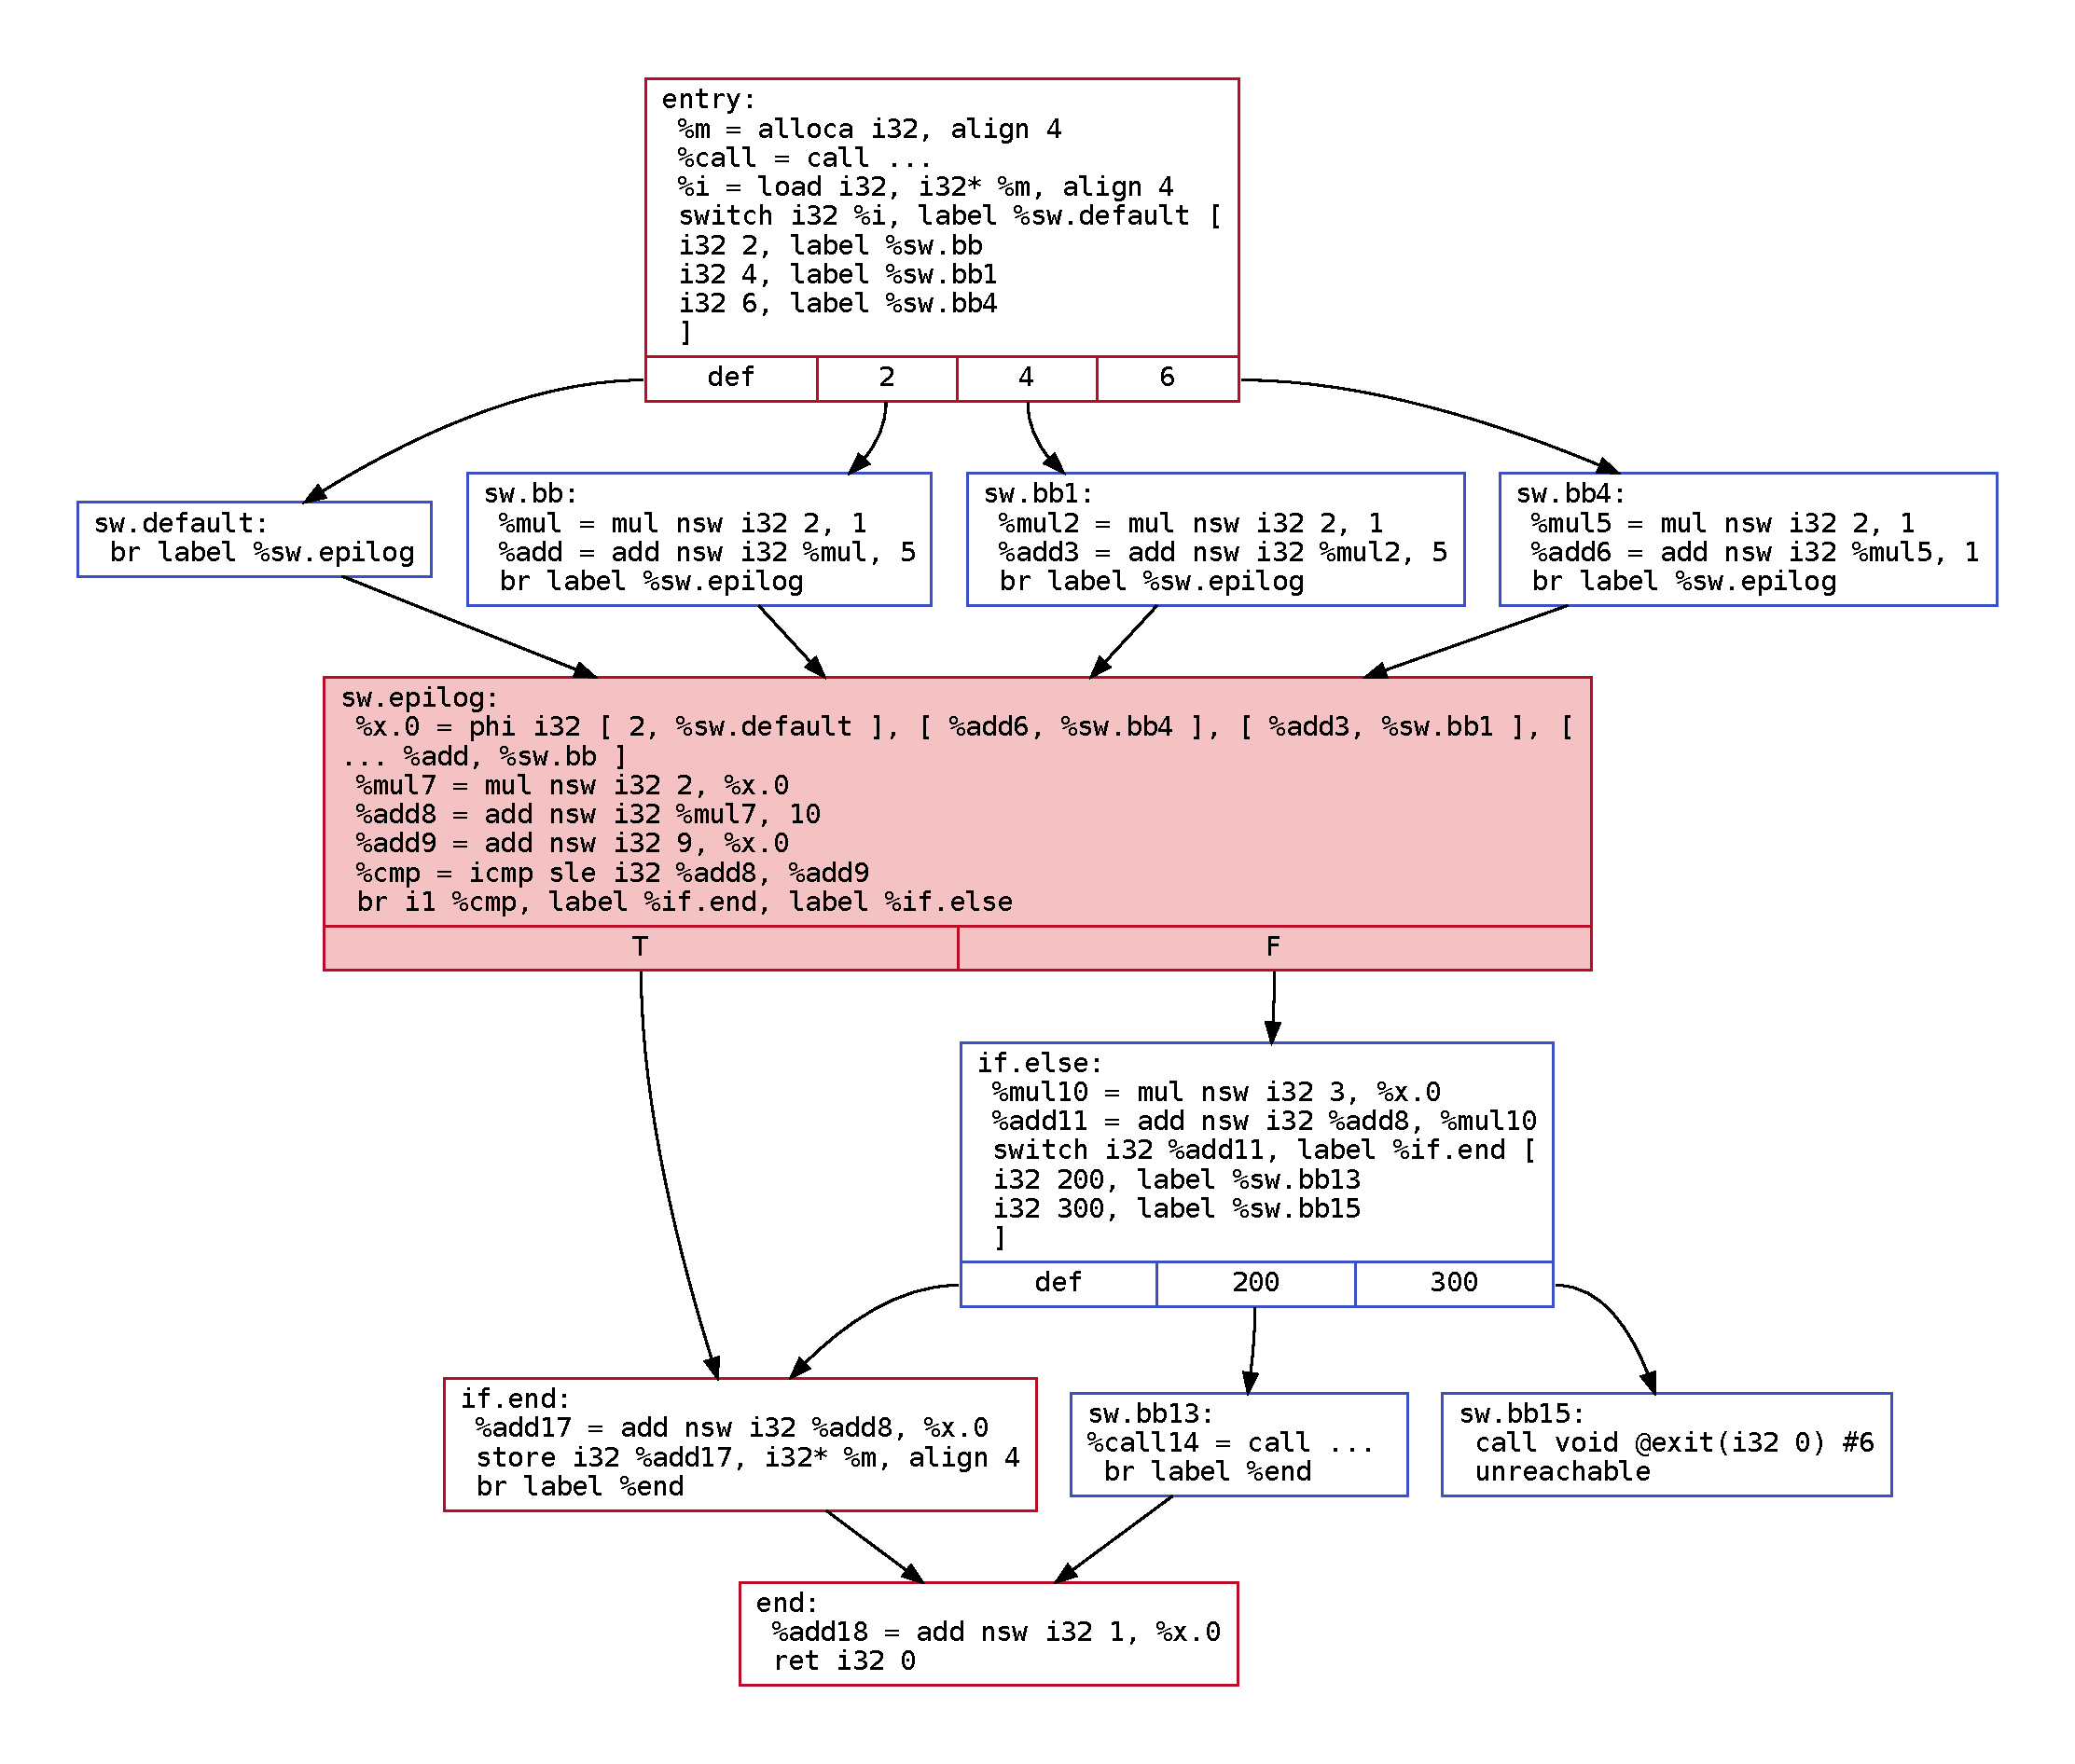
\includegraphics[width=8.5cm,height=7.81cm]{baseline.pdf}
\end{frame}

\begin{frame}{Hot Path SSA Form}
	\centering
	%Before and After HPSSA CFG, Tau Insert points and calls highlighted.
	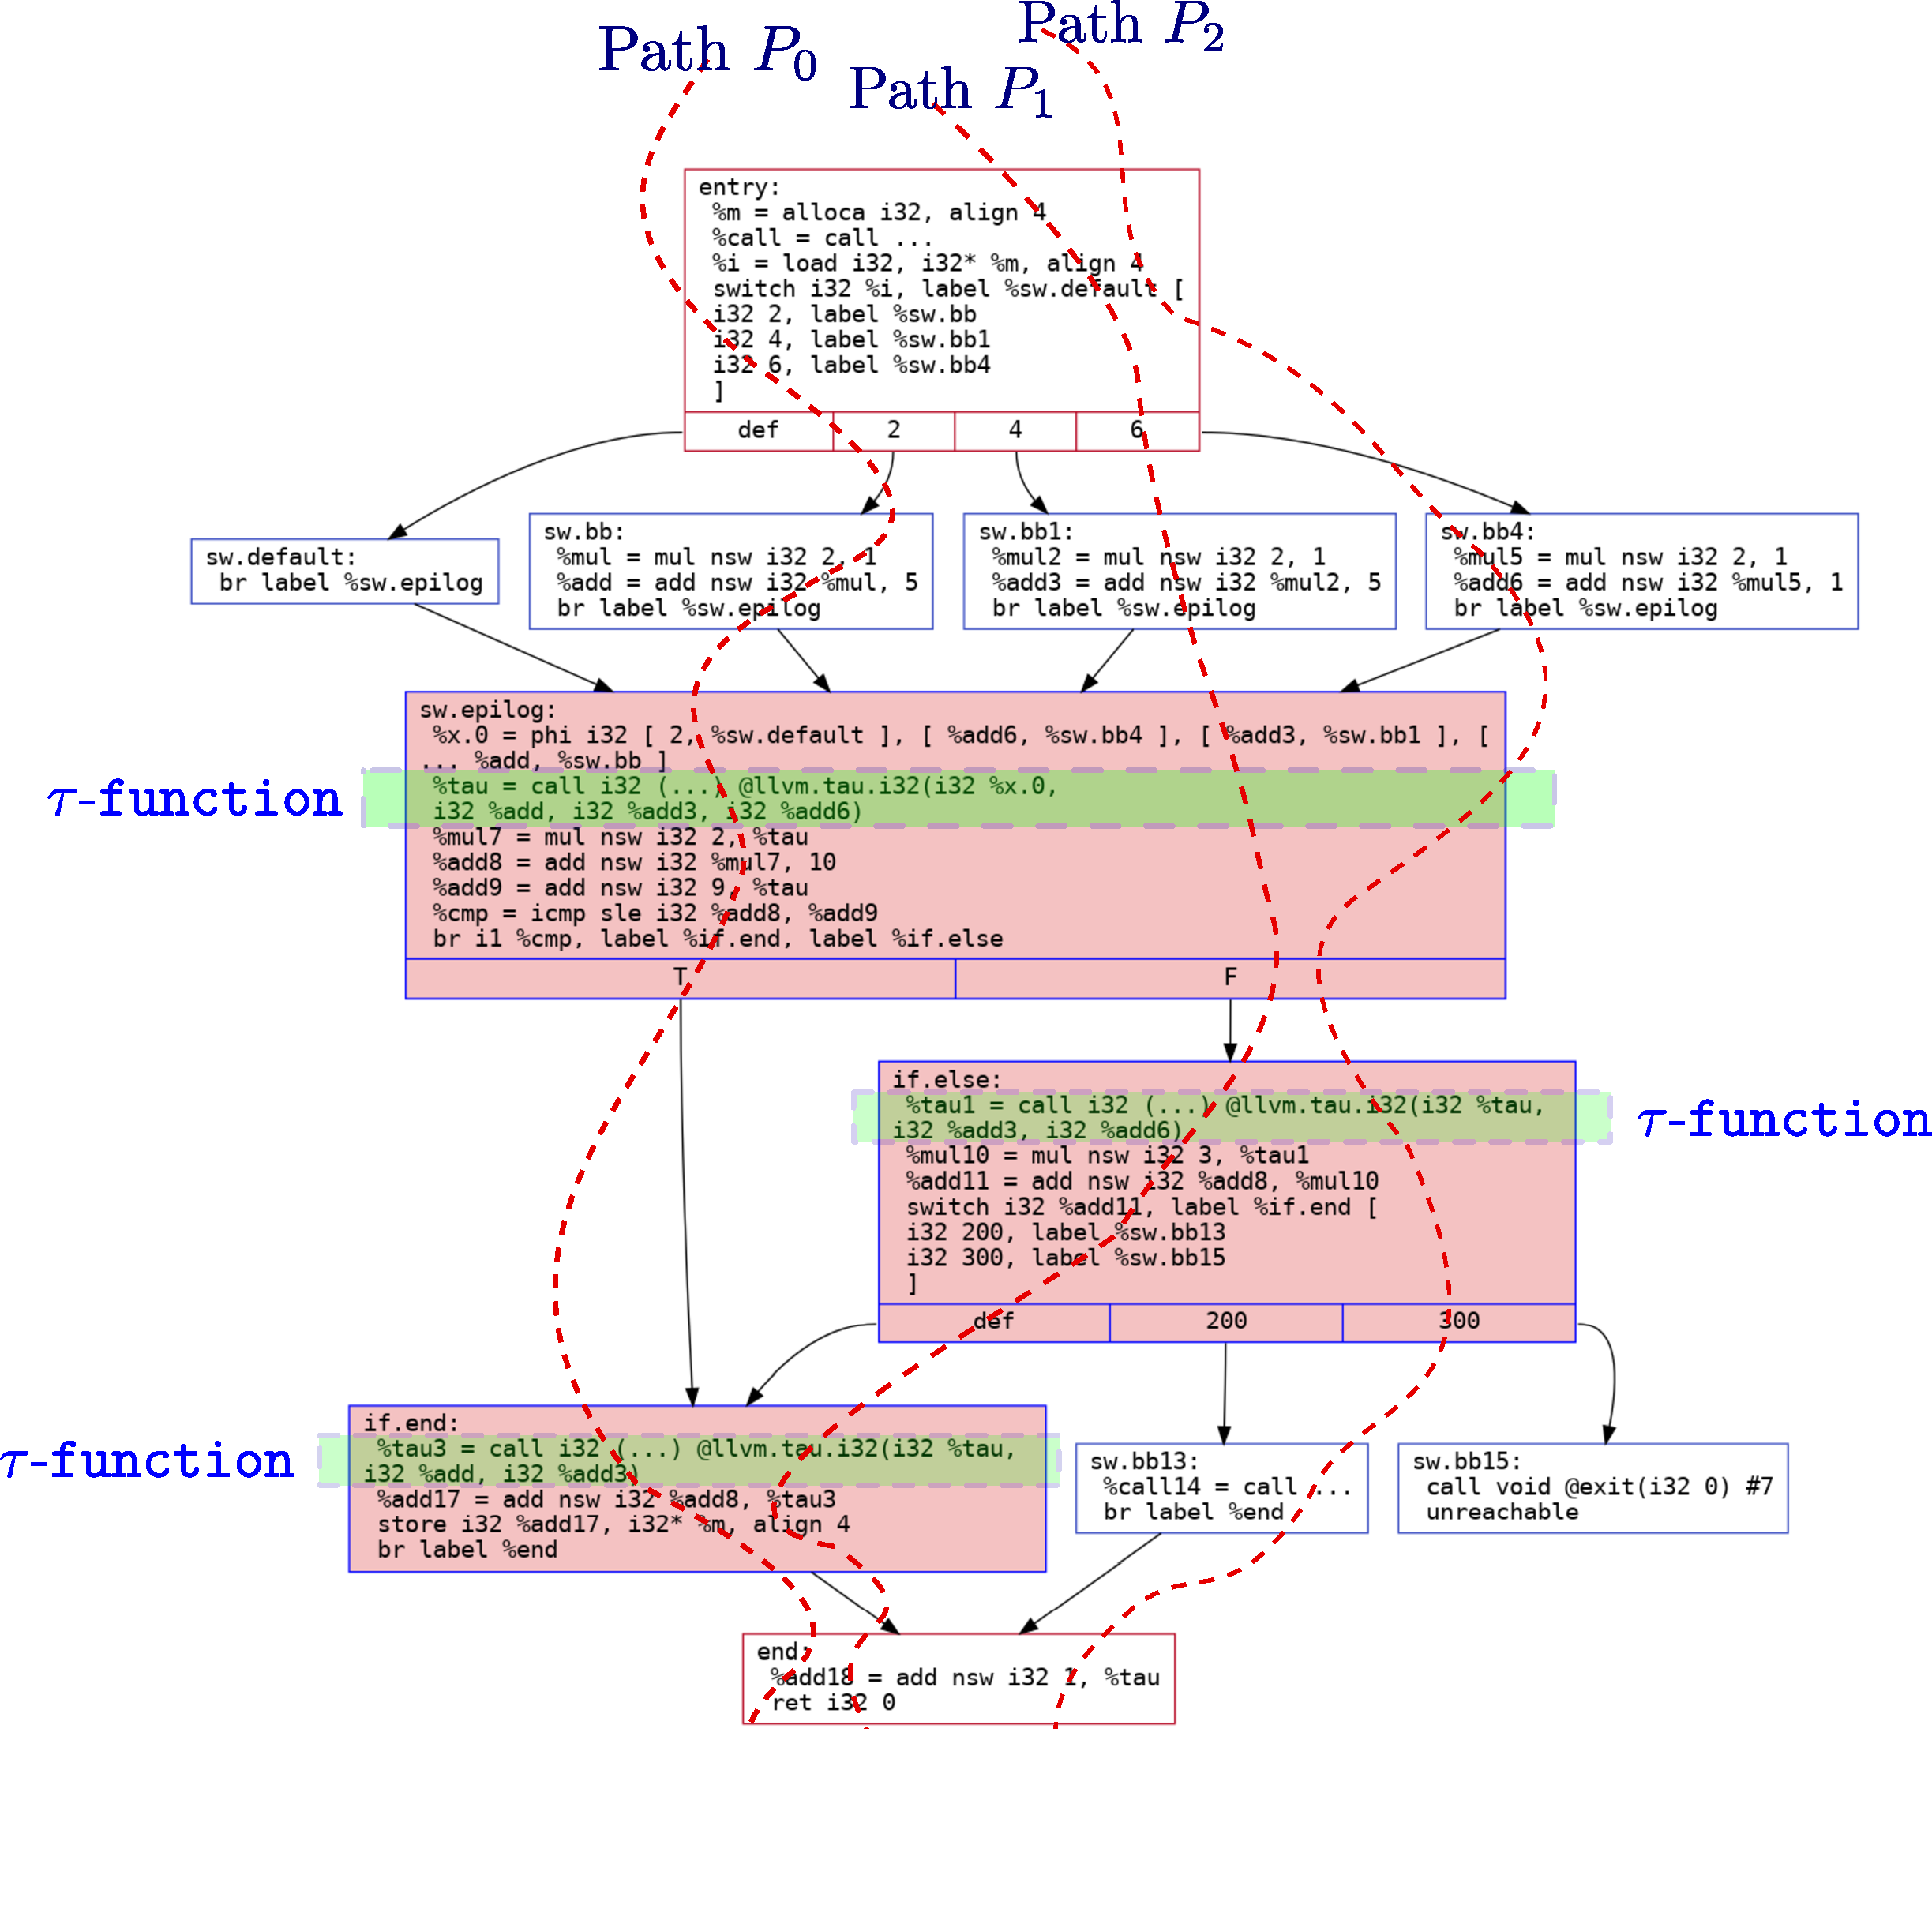
\includegraphics[width=8.5cm,height=8.35cm]{afterHPSSA.pdf}
\end{frame}

\begin{frame}
	\frametitle{\texttt{HPSSAPass} : Main Pass}
	\begin{itemize}
		\item \mintinline[fontsize=\footnotesize]{cpp}{HPSSAPass::run(Function &F, FunctionAnalysisManager &AM)} 
		\begin{itemize}
			\footnotesize
			\item Invoke \mintinline[fontsize=\footnotesize]{css}{HPSSAPass::getProfileInfo()} function to get a compact representation of all the profiled \color{red} hot paths \color{black} in the program and then call \mintinline[fontsize=\footnotesize]{css}{HPSSAPass::getCaloricConnector()} to get all the caloric connectors from the \color{red} hot path \color{black} information. This is a precursor to finding strategic positions to place \mintinline[]{css}{"llvm.tau"} intrinsic calls in the LLVM IR.
			\item Runs over each basic block in the function "F" in topological order using iterator returned from \mintinline[fontsize=\footnotesize]{css}{llvm::Function::RPOT()} call.
			\item Uses the \mintinline[fontsize=\footnotesize]{css}{llvm::dominates()} function from \mintinline[fontsize=\footnotesize]{css}{llvm::DominatorTreeAnalysis} to check for dominance frontier while processing the child nodes of the current basic block. This step is a part of correctly placing \mintinline[]{css}{"llvm.tau"} intrinsic calls in the LLVM IR. 
			\item Uses the renaming stack and \mintinline[]{css}{HPSSAPass::Search()} function to search and replace all use of PHI result operand with that returned by the \mintinline[]{css}{"llvm.tau"} intrinsic call.
		\end{itemize}
	\end{itemize}
\end{frame}

\begin{frame}
	\frametitle{\texttt{HPSSAPass} : Destruction Pass}
	\begin{itemize}
		\item Out of HPSSA Form. 
		\begin{itemize}
			\item A seperate pass using the new LLVM Pass Manager. \mintinline[]{css}{class TDSTRPass : public PassInfoMixin<TDSTRPass>}
			\item Using \mintinline[fontsize=\footnotesize]{css}{TDSTRPass::run(Function &F, ...)}, we replace all use of existing tau operands with first argument of  \mintinline[]{css}{"llvm.tau"} intrinsic (corresponds to the safe argument) and remove the \mintinline[]{css}{"llvm.tau"} intrinsic calll from the LLVM IR.
			\item The LLVM IR becomes identical to what it was before running the HPSSA Pass. 
		\end{itemize}
	\end{itemize}
\end{frame}

\footnotesize

\section{Conclusion}
\begin{frame}
	\frametitle{Conclusion}
\end{frame}
\footnotesize

\end{document}